\documentclass[conference]{IEEEtran}
\IEEEoverridecommandlockouts

% Required packages for IEEEtran
\usepackage{cite}
\usepackage{amsmath,amssymb,amsfonts}
\usepackage{algorithmic}
\usepackage{graphicx}
\usepackage{textcomp}
\usepackage{xcolor}

% Additional packages from your article (ensuring they do not interfere with IEEE margins)
\usepackage{subcaption}
\usepackage{pgfplots}
\pgfplotsset{compat=1.17}
\usepackage{tikz}
\usepackage{listings}
\usepackage{verbatim}
\usepackage[edges]{forest}
\usepackage{adjustbox}

% Do not load geometry or bookmark in IEEEtran
%\usepackage{geometry}
%\usepackage{bookmark}

\begin{document}

\title{Comparing Machine Learning and Deep Learning Models with Attention Mechanisms for Multiple Authorship Attribution\\
\thanks{Identify applicable funding agency here. If none, delete this.}
}

\author{
\IEEEauthorblockN{Richard Čerňanský}
\IEEEauthorblockA{\textit{Department Name}\\
\textit{Organization}\\
City, Country\\
email@example.com}
\and
\IEEEauthorblockN{Ing. Juraj Petrík}
\IEEEauthorblockA{\textit{Department Name}\\
\textit{Organization}\\
City, Country\\
email@example.com}
}

\maketitle

\begin{abstract}
Authorship attribution (AA) in source code is crucial for plagiarism detection, forensic analysis, and software maintenance—especially when author information is missing or ambiguous. This field is not as well explored as written communication AA, and there are new models to be tested on different sized datasets. This study compares traditional machine learning models, such as Random Forests trained on TF-IDF tokenized representations, with deep learning models, including BERT and an Attention-based Neural Network (AttentionNN), for the task of multiple authorship attribution. We evaluate different representations of source code, including raw tokenized text and Abstract Syntax Tree (AST) structures, to determine their effectiveness in distinguishing authorship. The models are tested on a dataset of 3,004 C language functions from Google Code Jam spanning 2009--2018, assessing their accuracy, precision, recall, and training efficiency across varying author set sizes. Our findings highlight the strengths and limitations of each approach, showing that while deep learning models, particularly BERT trained on raw source code, achieve the highest accuracy, Random Forests offer competitive results with significantly lower computational cost. The study also explores the impact of function complexity on model performance, revealing that AttentionNN benefits from structural complexity while struggling with short functions. The results emphasize the trade-offs between accuracy, computational efficiency, and data representation, providing insights into the optimal model selection for source code authorship attribution.
\end{abstract}

\begin{IEEEkeywords}
Authorship attribution, machine learning, deep learning, BERT, attention mechanisms, source code.
\end{IEEEkeywords}

\section{Introduction}

Authorship attribution in source code analysis is a crucial task with applications in plagiarism detection, forensic investigations, 
and intellectual property protection, as well as software maintenance and quality analysis when author information is missing, inaccurate, 
or ambiguous. Given a function written in a programming language, determining its author requires capturing distinct stylistic patterns. 
Traditional machine learning (ML) methods, such as Random Forests trained on TF-IDF tokenized representations, have shown promise in text-based 
authorship identification. However, recent advancements in deep learning (DL) have introduced transformer-based models, such as BERT, which leverage 
contextual embeddings and self-attention mechanisms to extract more meaningful patterns from textual data.

Despite the success of deep learning models in natural language processing (NLP), their application to source code authorship 
attribution across different dataset sizes remains relatively unexplored. Unlike natural language, source code exhibits a more 
rigid syntax and structure, making its representation a key challenge. Several approaches have been proposed—from direct tokenized 
representations of raw source code to abstract syntax tree (AST) transformations that capture program logic—but it remains unclear which 
representation is most effective for distinguishing authorship across various levels of dataset complexity.

This study systematically compares machine learning and deep learning models, including Random Forests, BERT trained on tokenized source code, 
BERT trained on AST representations, and an Attention-based Neural Network (AttentionNN) utilizing AST-derived node-to-node paths. The evaluation 
is conducted on a dataset of 3,004 C language functions from Google Code Jam (GCJ) spanning 2009 to 2018 \cite{gcj}. The models are assessed 
based on their accuracy, precision, recall, and training efficiency across different author set sizes. Through this comparison, we aim to 
determine which model best balances accuracy and computational efficiency, as well as the effectiveness of different function representations 
for authorship attribution.

\section{Methods}

\subsection{Source Code Representation}

In \cite{information}, the authors present a division of features based on the extraction method:
\begin{itemize}
    \item \textbf{Stylometric features:} Capture structural characteristics that represent an author’s preference for various statements, keywords, 
    and nesting sizes.
    \item \textbf{N-gram features:} Extract contiguous sequences of bytes, characters, or words using a fixed-length sliding window.
    \item \textbf{Graph-based features:} Capture underlying traits in the code such as deep nesting, control flow, and data flow. This includes 
    representations such as the AST, Program Dependency Graph (PDG), Control Flow Graph (CFG), and RFG.
    \item \textbf{Behavioral features:} Focus on the program’s runtime behavior (e.g., CPU and memory usage) and instruction-level features from binaries.
    \item \textbf{Neural Network Generated Representations:} Recently, neural networks have been used to generate embeddings of source code. This approach 
    is applied in this study by using AST analysis to provide input for the neural network.
\end{itemize}

\subsection{Abstract Syntax Tree (AST)}

Based on the definition in \cite{sun2023AST}, an Abstract Syntax Tree (AST) is a tree-based representation of source code where nodes represent elements of the code and edges represent the relationships between these elements. The AST is an essential component in the compilation process, serving as an intermediate representation used for optimization and machine code generation. Nodes in the AST can be either internal (non-leaf), which define the program's constructs, or leaf nodes, which store actual textual values.

Below is an example of a simple C function and its corresponding AST:

\begin{figure}[!t]
    \centering
    % C code listing in a minipage
    \begin{minipage}{\columnwidth}
    \begin{lstlisting}[caption={Simple C function for addition}, label={lst:add}, basicstyle=\footnotesize\ttfamily, frame=single, numbers=left]
    int add(int a, int b) {
        return a + b;
    }
    \end{lstlisting}
    \end{minipage}
    
    \vspace{1em} % Adjust vertical space between listing and diagram
    
    % AST diagram scaled to column width
    \resizebox{\columnwidth}{!}{%
    \begin{forest}
    for tree={
      font=\fontsize{14pt}{16pt}\selectfont,
      l sep=3cm,
    }
    [TranslationUnit
      [\textbf{FunctionDefinition}: {int add(int a, int b) \{}
        [\textbf{BasicTypeSpecifier}: {int}]
        [\textbf{FunctionDeclarator}: {add(}
          [\textbf{IdentifierDeclarator}: {add}]
          [\textbf{ParameterSuffix}: {(int a, int b)}
            [\textbf{ParameterDeclaration}: {int a}
              [\textbf{BasicTypeSpecifier}: {int}]
              [\textbf{IdentifierDeclarator}: {a}]
            ]
            [\textbf{ParameterDeclaration}: {int b}
              [\textbf{BasicTypeSpecifier}: {int}]
              [\textbf{IdentifierDeclarator}: {b}]
            ]
          ]
        ]
        [\textbf{CompoundStatement}: {\{ return a + b; \}}
          [\textbf{ReturnStatement}: {return a + b;}
            [\textbf{AddExpression}: {a + b}
              [\textbf{IdentifierName}: {a}]
              [\textbf{IdentifierName}: {b}]
            ]
          ]
        ]
      ]
    ]
    \end{forest}
    }
    \caption{(a) C function code listing and (b) corresponding AST diagram.}
    \label{fig:combined_ast}
\end{figure}

\subsubsection{AST --- Types of Features}

Features extracted from the AST fall into four main categories:
\begin{itemize}
    \item \textbf{Structural:} Capture the AST's complexity (e.g., depth, number of nodes, average branching factor).
    \item \textbf{Semantic:} Reflect semantic information such as the distribution of node types or distinct root-to-leaf paths.
    \item \textbf{Syntactic:} Describe the programming paradigm and logical complexity (e.g., number of functions, control flow units).
    \item \textbf{Combined:} Use-case specific features that combine the aforementioned strategies for tasks like authorship attribution or 
    function name classification.
\end{itemize}

\subsubsection{Halstead Complexity Measures}

To evaluate function complexity, we used Halstead complexity measures (Difficulty, Volume, Effort) as defined in \cite{halstead}. 
These measures were aggregated into a single value using a weighted sum with ratios 4:3:3. (Halstead length was not incorporated, as it was analyzed separately.)

\subsection{Our Data Representation}

For training the models, a prediction task data pipeline was constructed as follows:

\begin{figure}[!t]
    \centering
    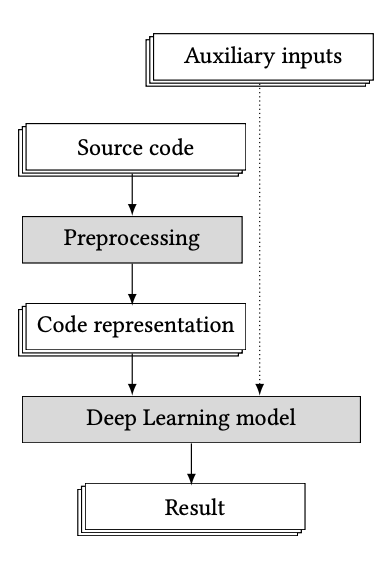
\includegraphics[width=3.5cm,height=5cm]{figures/high_level_prediciton_task.png}
    \caption{\cite{compiler_based} High-level overview of the function classification prediction task.}
    \label{fig:predictive_task}
\end{figure}

Various representations of each function’s raw source code were utilized:
\begin{itemize}
    \item Word-tokenized TF-IDF vectors for Random Forests.
    \item Byte Pair Encoding (BPE) of raw source code for BERT.
    \item Linearized AST pre-order traversal for BERT.
    \item A set of 600 randomly selected node-to-node paths for AttentionNN.
\end{itemize}
The PsycheC project's C language frontend parser \cite{psychec} was used to convert code into ASTs. Models were trained in the 
TensorFlow.Keras framework using different author set sizes (110, 27, 11, and 3) with minimum function counts per author of 25, 40, 50, and 58 respectively.

\subsection{Data Preprocessing \& Exploratory Data Analysis}

The dataset consisted of thousands of solutions from hundreds of authors. From each solution, the function and its author were extracted. 
The largest dataset comprised $3\,004$ C language functions from GCJ solutions (2009--2018). Preprocessing involved duplicate removal,
elimination of authors with disproportionately many samples, and exclusion of functions that could not be parsed into an AST. Frequency 
distributions of authors and function lengths were analyzed for further insights.


\begin{table*}[!t]
    \renewcommand{\arraystretch}{1.3}
    \caption{Comparison of models across author attribution accuracy and training time for different author set sizes.}
    \label{tab:comparison}
    \centering
    \begin{tabular}{lcccc}
    \hline
    \multicolumn{5}{c}{\textbf{Model Performance on Author Set Sizes}} \\
    \hline
    \textbf{Model} & \textbf{110} & \textbf{27} & \textbf{11} & \textbf{3} \\
    \hline
    Random Forests (TF-IDF) & 66.24\% / 3.63 min & 70.60\% / 0.23 min & 80.56\% / 0.08 min & 85.84\% / 0.05 min \\
    BERT (source code)    & 72.47\% / 30.33 min & 82.72\% / 9.49 min & 89.84\% / 5.30 min  & \textbf{90.70\% / 1.82 min} \\
    BERT (AST traversal)  & 24.07\% / 33.53 min & 35.66\% / 10.30 min & 40.62\% / 6.20 min  & 83.72\% / 1.22 min \\
    AttentionNN (AST paths)& 36.93\% / 3.53 min  & 53.42\% / 1.19 min  & 60.82\% / 0.54 min  & 69.30\% / 0.19 min \\
    \hline
    \end{tabular}
\end{table*}

\begin{figure}[!t]
    \centering
    \begin{subfigure}{0.48\textwidth}
        \centering
        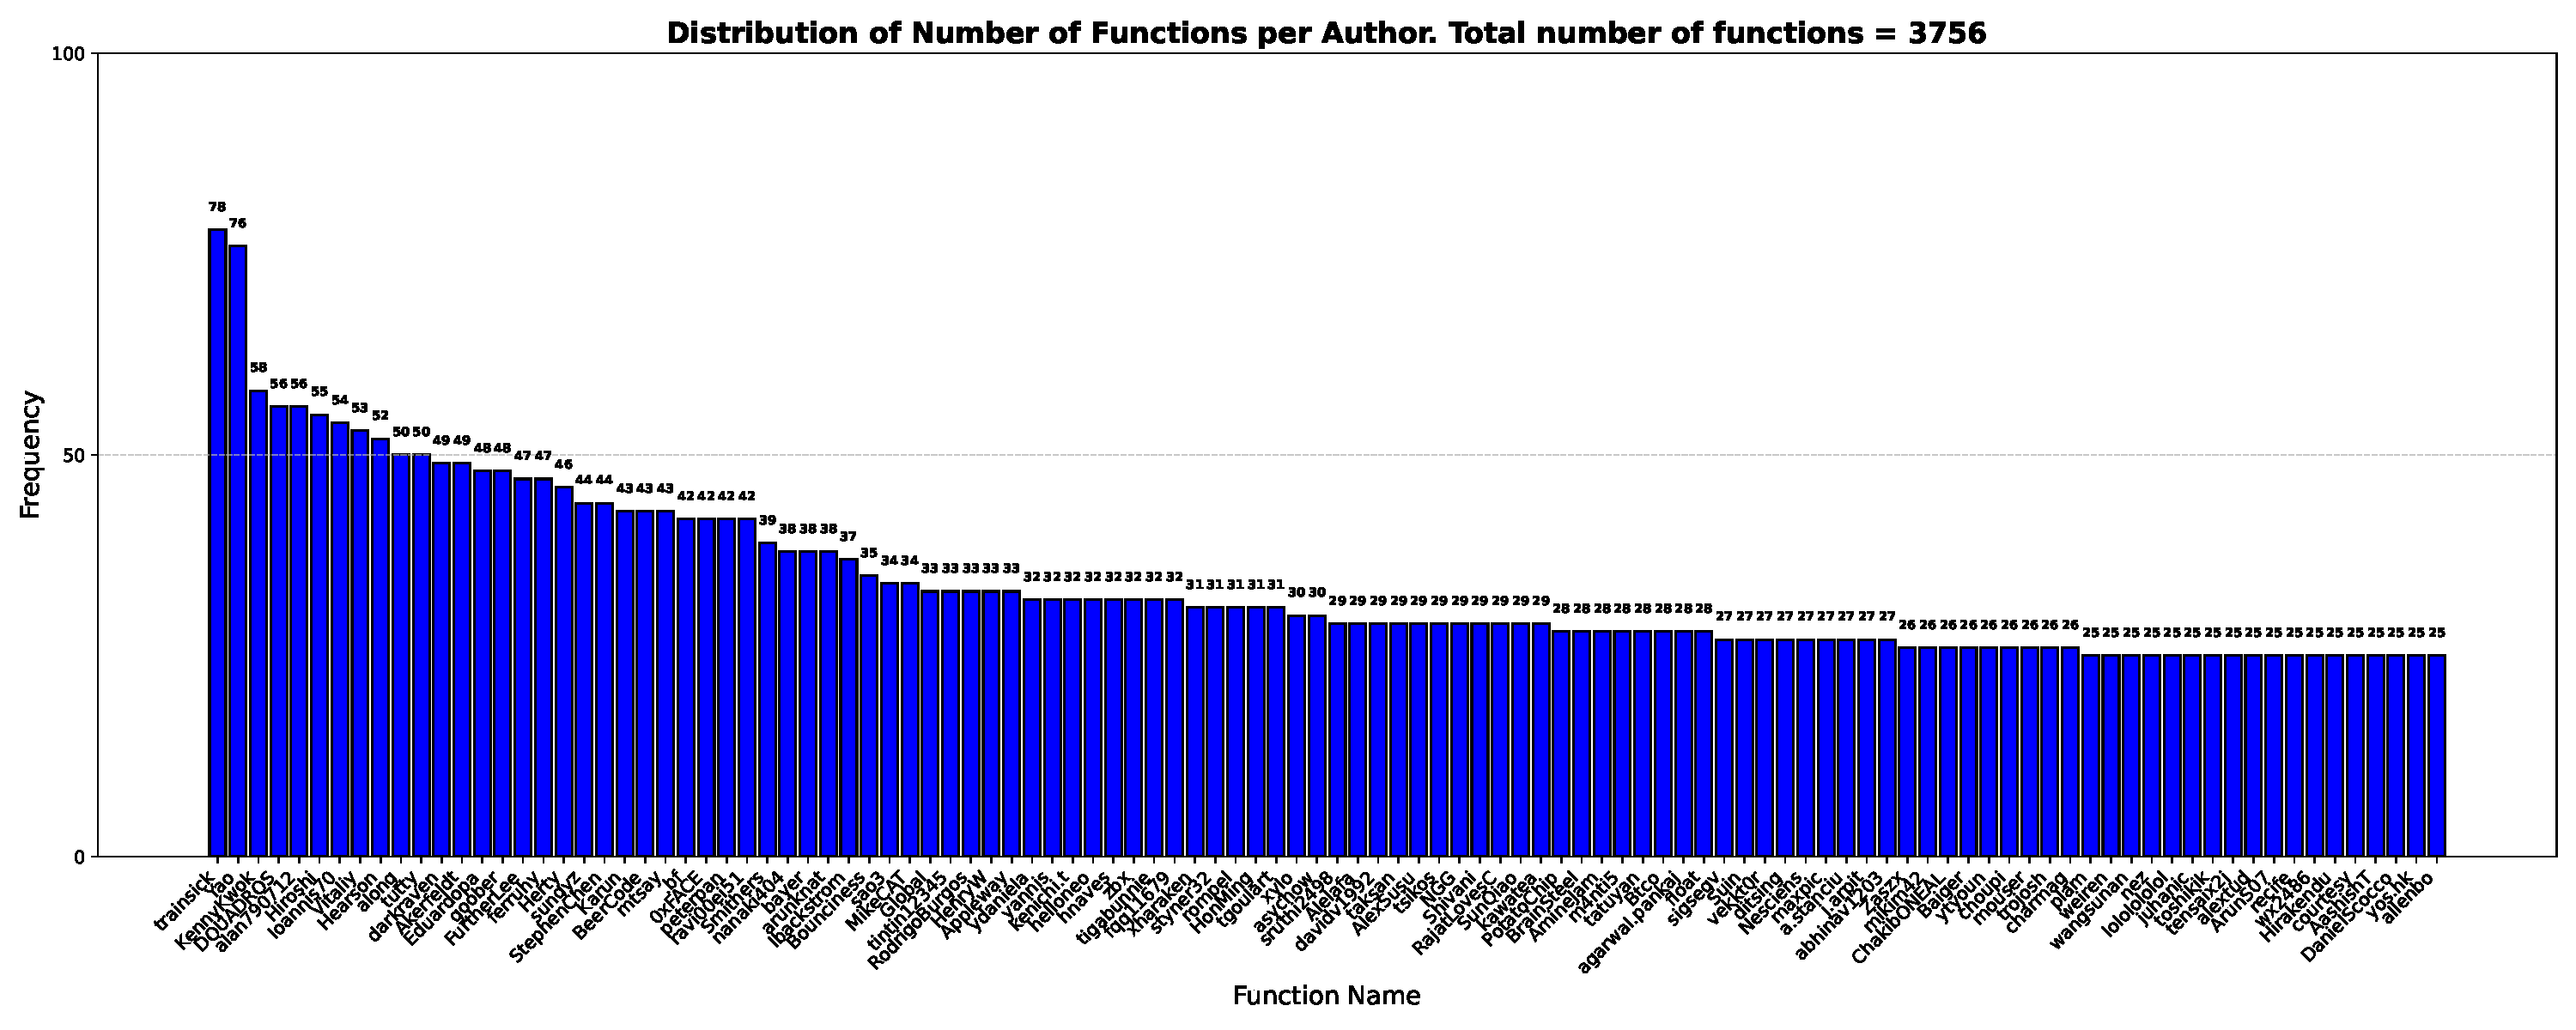
\includegraphics[width=\linewidth]{figures/distribution_names.pdf}
        \caption{Frequency distribution of author names}
        \label{fig:distr_names}
    \end{subfigure}
    \hfill
    \begin{subfigure}{0.48\textwidth}
        \centering
        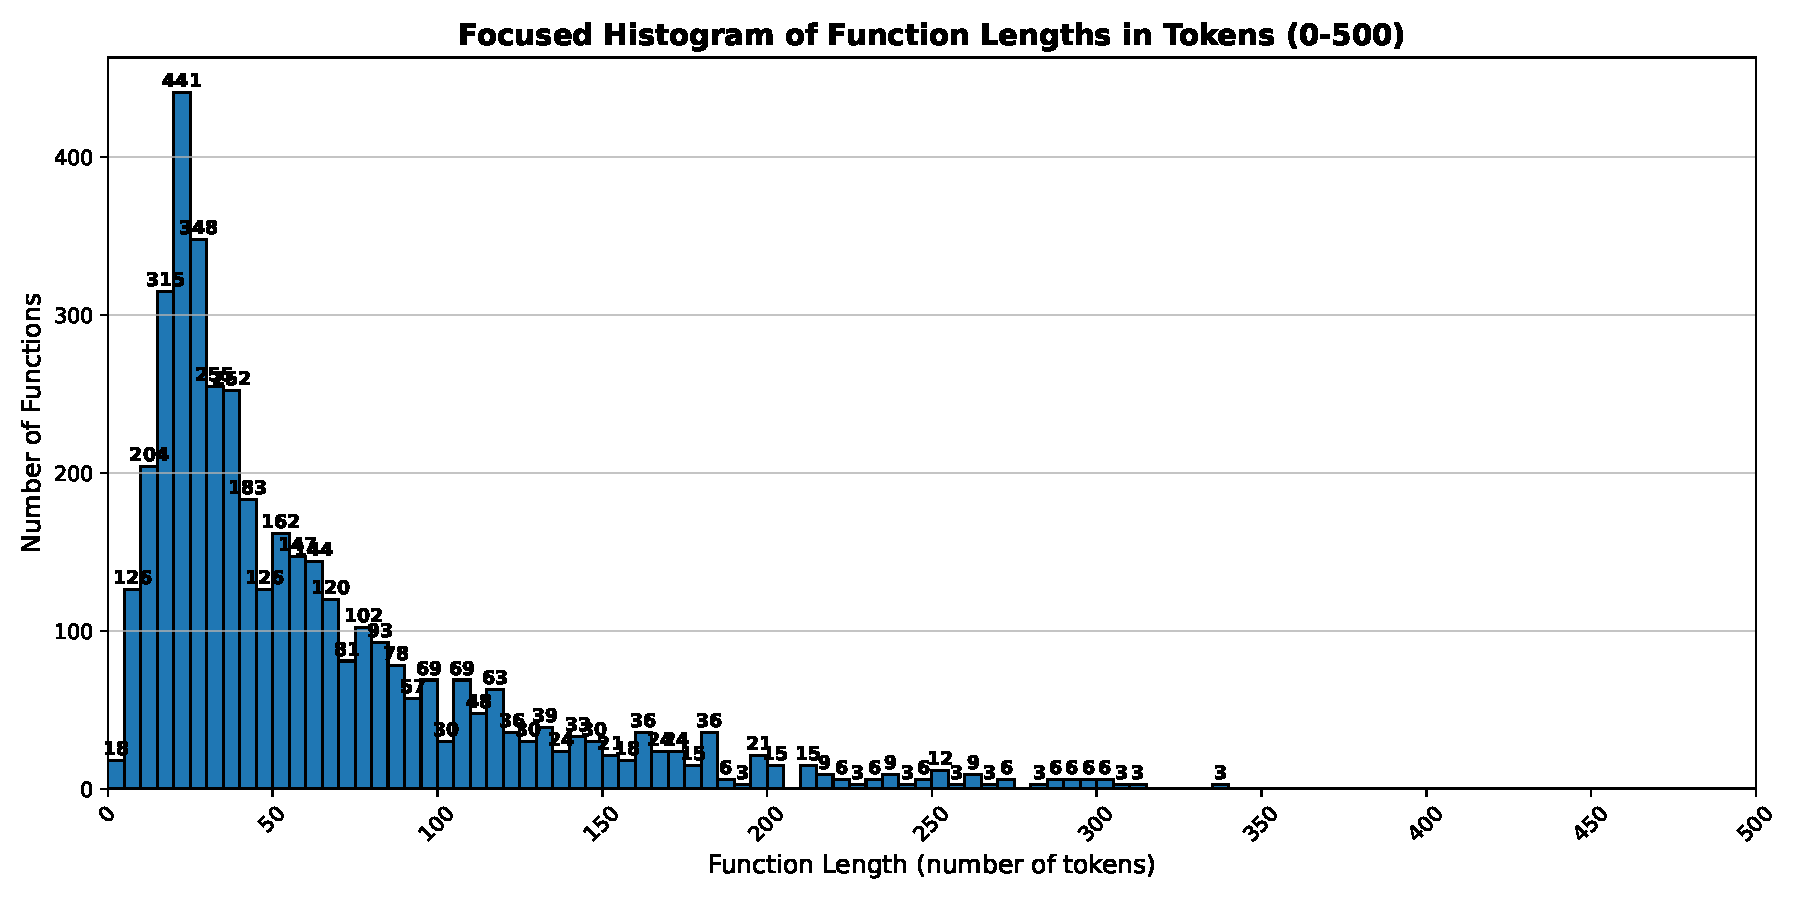
\includegraphics[width=\linewidth]{figures/distr_lens_tokens.pdf}
        \caption{Frequency distribution of function lengths}
        \label{fig:disrt_lens}
    \end{subfigure}
    \caption{Important frequency distributions of our dataset.}
    \label{fig:eda_distr}
\end{figure}

Figure~\ref{fig:distr_names} shows that most function lengths are between 10 and 50 tokens, 
making single-function authorship attribution challenging when only short code snippets are available.

\section{Models Setup \& Training}

Random Forests and AttentionNN models were trained using a stratified cross-validation strategy (5 folds: 3 for training,
 1 for validation, and 1 for testing). Because BERT training requires considerably more time, it was repeated three times, with evaluation metric variance below 1\%.

\subsection{Random Forests}
Random Forests were chosen as a baseline for text-based authorship attribution. They were trained on word-level tokens (using the regex \verb|r"\b\w+\b"|). A grid search was performed to optimize hyperparameters:
\begin{itemize}
    \item \textbf{n\_estimators}: \{50, 100, 200, 500\}
    \item \textbf{max\_depth}: \{10, 20, 30, None\}
    \item \textbf{min\_samples\_split}: \{2, 5, 10\}
    \item \textbf{min\_samples\_leaf}: \{1, 2, 4\}
    \item \textbf{max\_features}: \{"sqrt", "log2", None\}
    \item \textbf{bootstrap}: \{True, False\}
\end{itemize}
The best hyperparameters were then used to train the final model.

\subsection{BERT}
For both BERT setups, Microsoft’s pretrained \texttt{graphcodebert-base} \cite{codebert} was used. The graphcodebert tokenizer uses Byte Pair Encoding, which is suitable for programming languages with rigid syntax. Comments were removed to ensure fairness when comparing models that utilize ASTs. BERT was trained on two distinct representations: tokenized raw source code and tokenized AST pre-order traversal.

\subsection{Attention Neural Network}
The AttentionNN model leverages AST-derived node-to-node paths (path-contexts) as proposed in \cite{code2vec}. Each path is represented as a triplet (start node, path of node kinds, terminal node) and encoded into vector space. The model then learns to weigh these contexts via an attention mechanism to distinguish authors.

\subsection{Evaluation Methods}
Evaluation metrics included validation accuracy, precision, recall, training time, and Halstead complexity measures. Deep learning models were trained with the categorical cross-entropy loss function:
\begin{equation}
    \mathcal{L}_i = - \sum_{j=1}^{C} y_{i,j} \log(\hat{y}_{i,j})
\end{equation}
where:
\begin{itemize}
    \item $\mathcal{L}_i$ is the loss for sample $i$.
    \item $C$ is the number of classes.
    \item $y_{i,j}$ is the one-hot encoded ground truth for class $j$.
    \item $\hat{y}_{i,j}$ is the predicted probability for class $j$ (obtained from a softmax function).
\end{itemize}
Learning curves were analyzed to assess overfitting. The overfit ratio was calculated as:
\begin{equation}
    \text{Overfit Ratio} = \frac{\text{Train Accuracy}}{\text{Test Accuracy}}
\end{equation}


\begin{figure*}[!t]
    \centering
    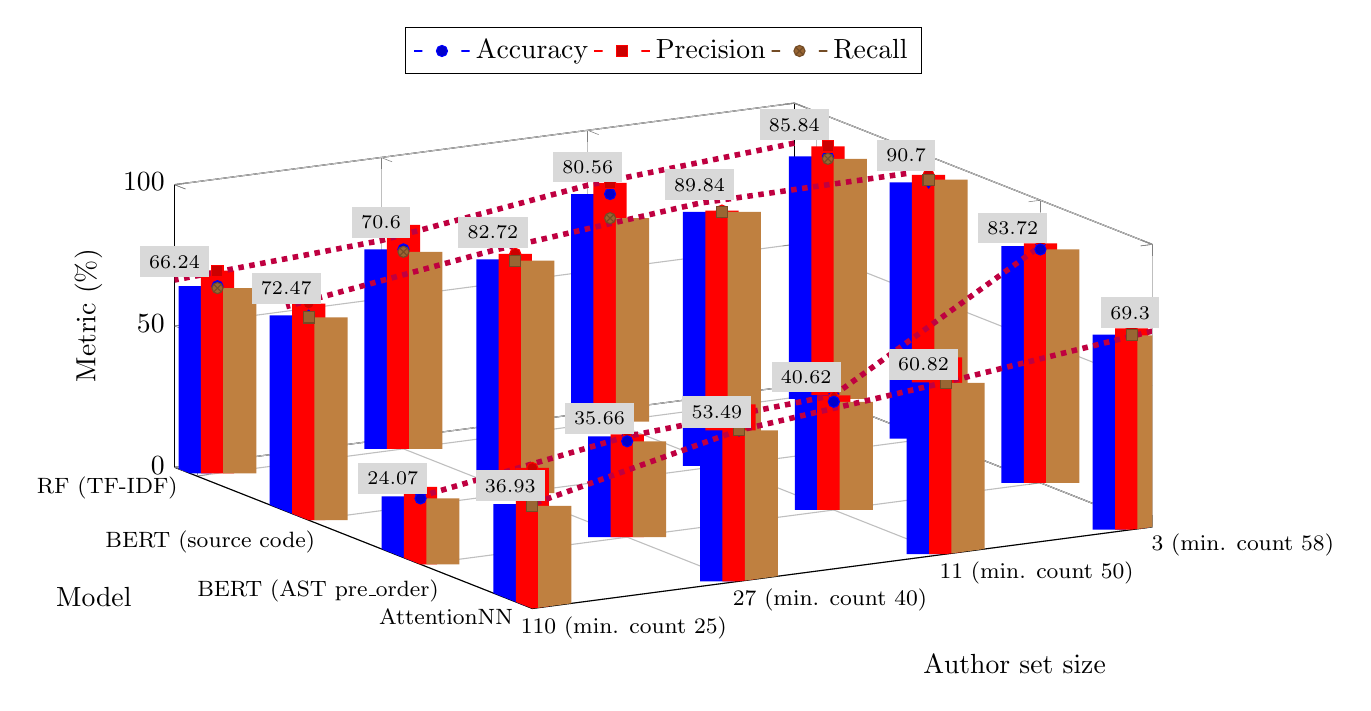
\begin{tikzpicture}
    \begin{axis}[
        view={60}{30},
        z buffer=sort,
        xlabel={Model},
        xlabel style={xshift=-40pt,yshift=40pt,align=center},
        ylabel={Author set size},
        ylabel style={xshift=25pt,yshift=20pt,align=center},
        zlabel={Metric (\%)},
        width=14cm,
        height=8cm,
        xtick={1,2,3,4},
        xticklabels={RF (TF-IDF), BERT (source code), BERT (AST pre\_order), AttentionNN},
        xticklabel style={font=\footnotesize,xshift=-20pt,yshift=10pt,align=center},
        ytick={4,3,2,1},
        yticklabels={3 (min. count 58), 11 (min. count 50), 27 (min. count 40), 110 (min. count 25)},
        yticklabel style={font=\footnotesize,xshift=25pt,yshift=5pt,align=center},
        zmin=0, zmax=100,
        grid=major,
        legend style={at={(0.5,1.15)},anchor=north,legend columns=3}
    ]
    
    % MODEL 1: RF (x = 1)
    \addplot3+[ybar, bar width=12pt, fill=blue, draw=none, bar shift=-0.2]
        coordinates {(1.1,4,85.84) (1,3,80.56) (1,2,70.60) (1,1.1,66.24)};
    \addplot3+[ybar, bar width=12pt, fill=red, draw=none, bar shift=0]
        coordinates {(1.1,4,89.36) (1,3,84.56) (1,2,79.27) (1,1.1,71.73)};
    \addplot3+[ybar, bar width=12pt, fill=brown, draw=none, bar shift=+0.2]
        coordinates {(1.1,4,84.96) (1,3,72.03) (1,2,69.73) (1,1.1,65.55)};
    \addplot3+[mark=none, purple, dotted, line width=2pt, nodes near coords,
        every node near coord/.append style={mark=none, fill=gray!30, draw=none, text=black, font=\scriptsize,yshift=0pt}]
        coordinates {(0.8,4,85.84) (0.8,3,80.56) (0.8,2,70.60) (0.8,1,66.24)};
    
    % MODEL 2: BERT (source code) (x = 2)
    \addplot3+[ybar, bar width=12pt, fill=blue, draw=none, bar shift=-0.2]
        coordinates {(2,4,90.70) (2,3,89.84) (2,2,82.72) (2,1,72.47)};
    \addplot3+[ybar, bar width=12pt, fill=red, draw=none, bar shift=0]
        coordinates {(2,4,93.33) (2,3,90.33) (2,2,84.66) (2,1,76.69)};
    \addplot3+[ybar, bar width=12pt, fill=brown, draw=none, bar shift=+0.2]
        coordinates {(2,4,91.67) (2,3,89.92) (2,2,82.25) (2,1,71.76)};
    \addplot3+[mark=none, purple, dotted, line width=2pt, nodes near coords,
        every node near coord/.append style={mark=none, fill=gray!30, draw=none, text=black, font=\scriptsize,yshift=0pt}]
        coordinates {(1.8,4,90.70) (1.8,3,89.84) (1.8,2,82.72) (1.8,1,72.47)};
    
    % MODEL 3: BERT (AST pre_order) (x = 3)
    \addplot3+[ybar, bar width=12pt, fill=blue, draw=none, bar shift=-0.2]
        coordinates {(3,4,83.72) (3,3,40.62) (3,2,35.66) (3,1,24.07)};
    \addplot3+[ybar, bar width=12pt, fill=red, draw=none, bar shift=0]
        coordinates {(3,4,84.72) (3,3,40.53) (3,2,36.41) (3,1,27.40)};
    \addplot3+[ybar, bar width=12pt, fill=brown, draw=none, bar shift=+0.2]
        coordinates {(3,4,82.58) (3,3,38.30) (3,2,33.93) (3,1,23.33)};
    \foreach \yA/\zA/\yB/\zB in {
        4/83.72/3/40.62,
        3/40.62/2/35.66,
        2/35.66/1/24.07
    } {
        \addplot3+[mark=none, purple, dotted, line width=2pt, nodes near coords,
            every node near coord/.append style={mark=none, fill=gray!30, draw=none, text=black, font=\scriptsize,yshift=0pt,xshift=-10pt}]
        coordinates {(3,\yA,\zA) (3,\yB,\zB)};
    }
    
    % MODEL 4: AttentionNN (x = 4)
    \addplot3+[ybar, bar width=12pt, fill=blue, draw=none, bar shift=-0.2]
        coordinates {(4,3.9,69) (4,3,60.82) (4,2,53.42) (4,1,36.93)};
    \addplot3+[ybar, bar width=12pt, fill=red, draw=none, bar shift=0]
        coordinates {(4,3.9,71.25) (4,3,69.6) (4,2,62.6) (4,1,49.73)};
    \addplot3+[ybar, bar width=12pt, fill=brown, draw=none, bar shift=+0.2]
        coordinates {(4,3.9,68.76) (4,3,60.61) (4,2,53.45) (4,1,36.34)};
    \foreach \yA/\zA/\yB/\zB in {
        4/69.3/3/60.82,
        3/60.82/2/53.42,
        2/53.49/1/36.93
    } {
        \addplot3+[mark=none, purple, dotted, line width=2pt, nodes near coords,
            every node near coord/.append style={mark=none, fill=gray!30, draw=none, text=black, font=\scriptsize,yshift=0pt,xshift=-8pt}]
        coordinates {(4,\yA,\zA) (4,\yB,\zB)};
    }
    
    % LEGEND
    \addplot3+[ybar, fill=blue, draw=none, bar width=12pt, legend image code/.code={
        \draw[fill=blue] (0cm,-0.1cm) rectangle (0.6cm,0.1cm);
    }] coordinates {(0,0,-9999)};
    \addlegendentry{Accuracy}
    
    \addplot3+[ybar, fill=red, draw=none, bar width=12pt, legend image code/.code={
        \draw[fill=red] (0cm,-0.1cm) rectangle (0.6cm,0.1cm);
    }] coordinates {(0,0,-9999)};
    \addlegendentry{Precision}
    
    \addplot3+[ybar, fill=brown, draw=none, bar width=12pt, legend image code/.code={
        \draw[brown, mark=x] plot coordinates {(0cm,0cm)};
    }] coordinates {(0,0,-9999)};
    \addlegendentry{Recall}
    
    \end{axis}
    \end{tikzpicture}
    \caption{3D bar chart comparing Accuracy, Precision, and Recall across models and author set sizes.}
    \label{fig:3d-bars}
\end{figure*}


    
\section{Results}

The models were evaluated for scalability as the number of functions per author increased while the distinct author set size decreased. Table~\ref{tab:comparison} summarizes model performance (accuracy and training time) for various author set sizes.

Figure~\ref{fig:conf_matrix_bert} shows the confusion matrix for the best performing model (BERT on raw source code) for an author set size of 27.

\begin{figure}[!b]
    \centering
    \hspace*{-25pt}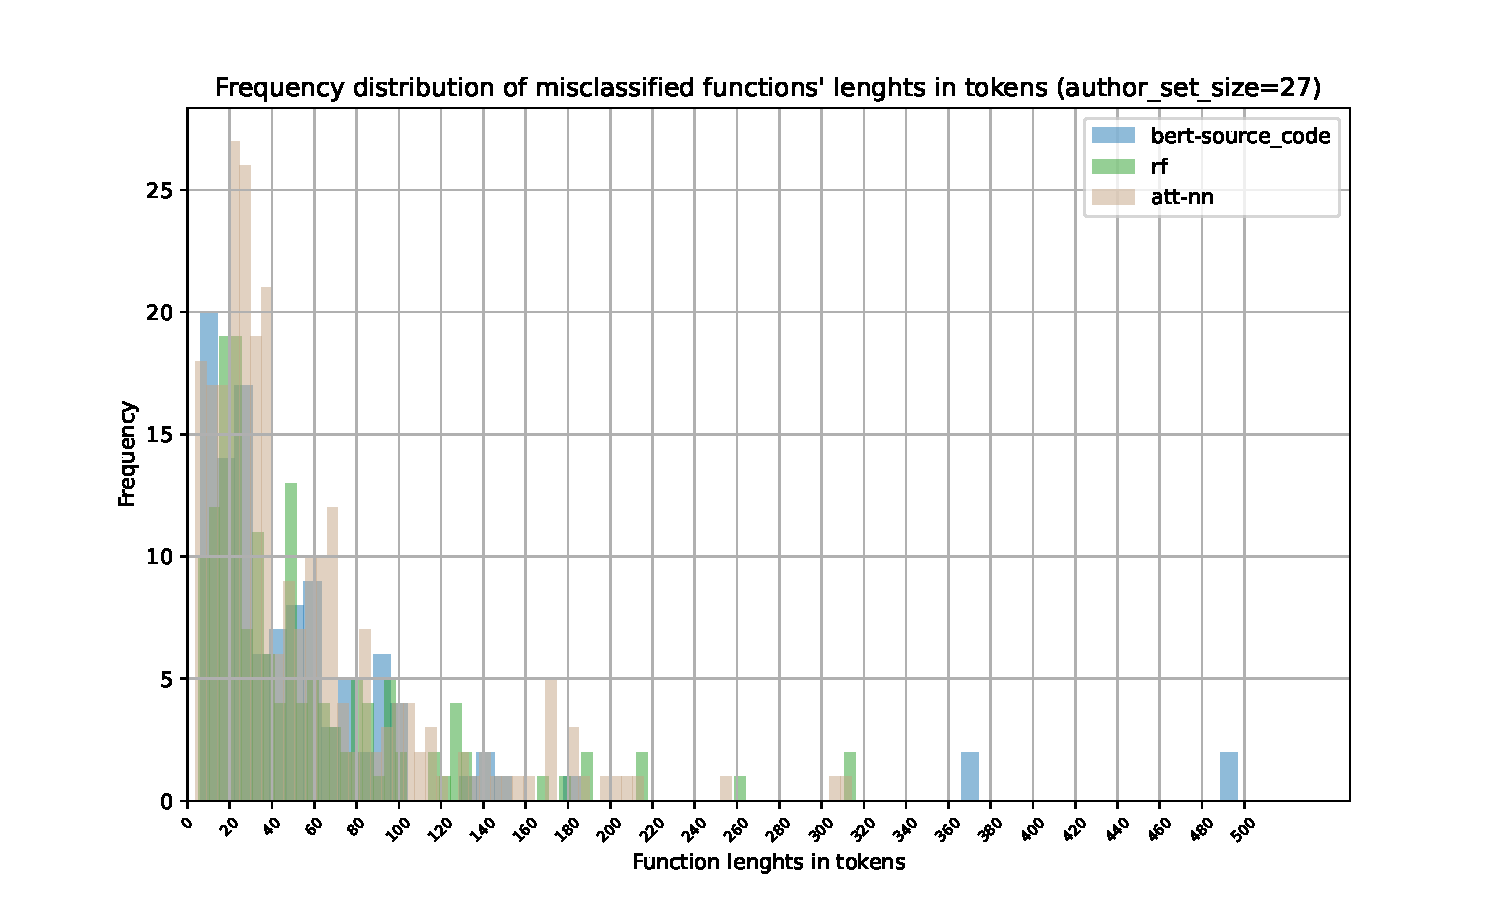
\includegraphics[width=1.2\columnwidth]{figures/misclass_lens.pdf}
    \caption{Frequency distribution of misclassified function lengths (in tokens) for Random Forests, BERT, and AttentionNN.}
    \label{fig:misclass_lens}
\end{figure}

We also analyzed the effect of function complexity. Figure~\ref{fig:misclass_lens} visualizes the frequency distribution of misclassified function lengths (in tokens) for Random Forests, BERT, and AttentionNN after scaling each model’s misclassification count by an index:
\begin{equation}
    \text{index}_{i} = \frac{\text{Number of misclassifications of the worst performing model}}{\text{Number of misclassifications of model } i}
\end{equation}

Figure~\ref{fig:misclass_halstead} shows the distribution of misclassified function Halstead complexity for Random Forests and BERT, revealing that while Random Forests struggle with higher complexity, BERT exhibits more misclassifications when complexity is low.

\begin{figure}[!b]
    \centering
    \hspace*{-25pt}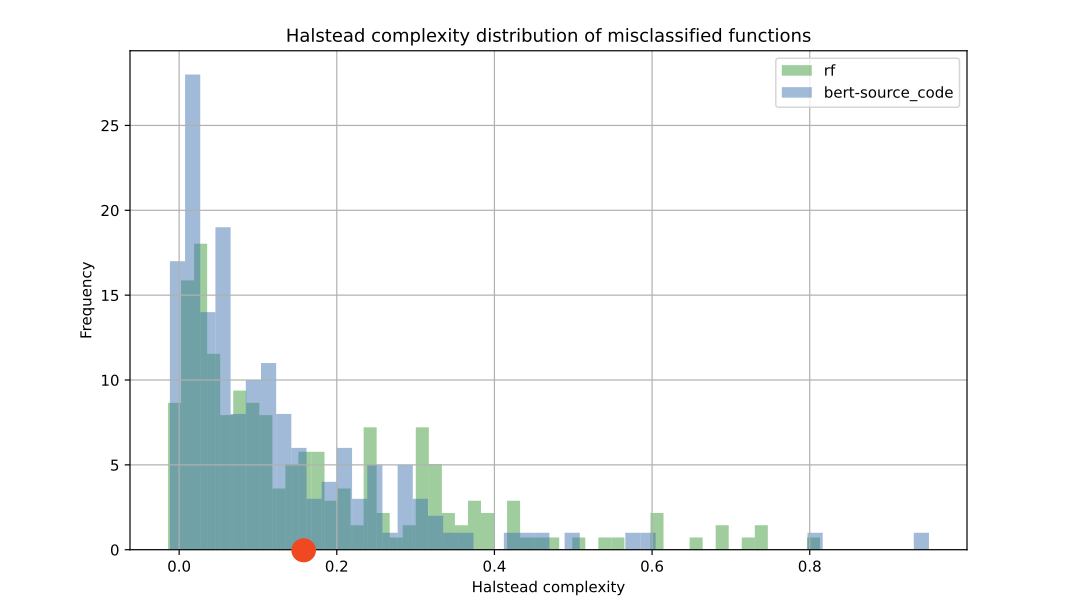
\includegraphics[width=1.2\columnwidth]{figures/misclass_hs.png}
    \caption{Frequency distribution of misclassified function Halstead complexity for Random Forests and BERT.}
    \label{fig:misclass_halstead}
\end{figure}

Furthermore, we assessed the AttentionNN model’s performance based on function complexity by evaluating accuracy across bins of AST node count and AST depth. Figure~\ref{fig:eda_distr} presents subfigures for these two metrics, indicating that the model learns better from structurally complex functions.

A 3D bar chart (Figure~\ref{fig:3d-bars}) further visualizes Accuracy, Precision, and Recall across models and author set sizes. (The code for this chart uses TikZ and pgfplots.)

\begin{figure}[!t]
    \centering
    % Scale to the column width (100%)
    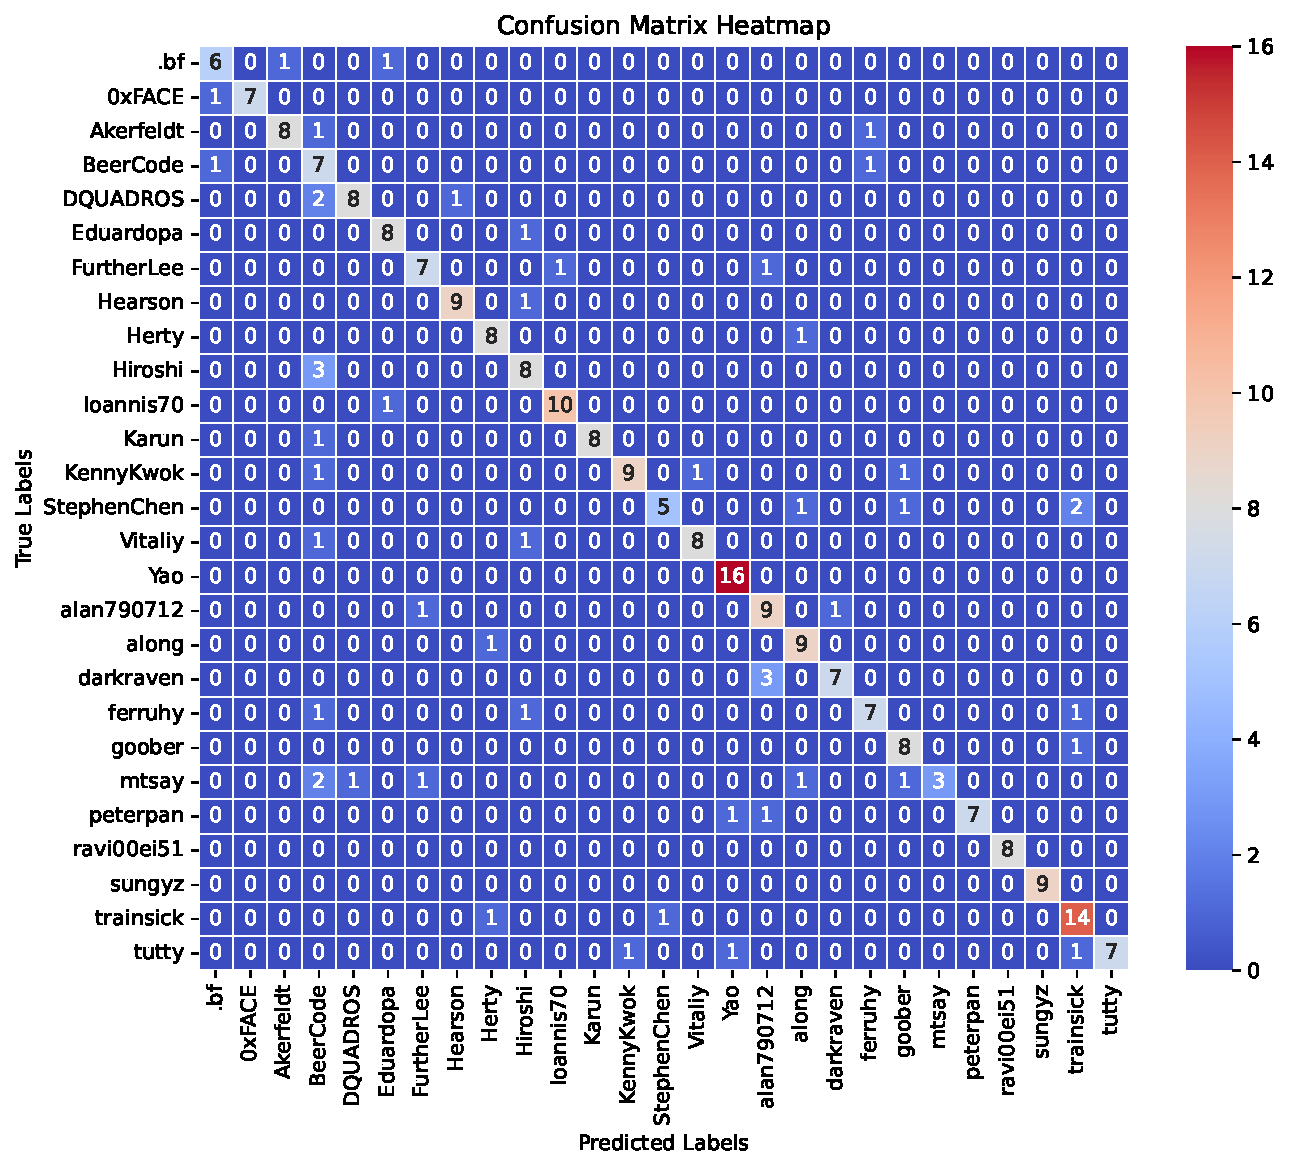
\includegraphics[width=\columnwidth]{figures/conf_matrix_sourcode_bert_ts27.pdf}
    \caption{Confusion matrix for BERT trained on raw source code (author set size 27).}
    \label{fig:conf_matrix_bert}
\end{figure}

\section{Discussion}

Our findings show that deep learning models, especially BERT, perform better than traditional machine learning methods for authorship attribution 
of single functions. But this comes at a cost—BERT needs way more computation and training time. On the other hand, Random Forest with TF-IDF 
tokenization held up surprisingly well, especially with larger author sets, and trained very fast.

A key takeaway is that BERT trained on raw source code tokens consistently had the best accuracy across all dataset sizes. However, 
its improvement from \texttt{set\_size=11} to \texttt{set\_size=3} was only 0.86\%, meaning increasing the minimum function count per author 
after a certain point doesn’t do much. Interestingly, BERT using AST pre-order traversal struggled with large author sets but got way better 
when we reduced the dataset to three authors. This shows how important it is to choose the right input representation for deep learning models.

Looking at misclassifications, each model had its weak points. BERT had trouble with short functions that had low Halstead complexity— they 
don’t provide enough meaningful context to determine the author. Random Forests, which rely more on statistical patterns than contextual 
understanding, started failing as function complexity increased. This makes sense since TF-IDF representations capture token frequency but 
don’t really understand code structure.

AttentionNN, which works with AST-derived node-to-node paths, preferred structurally complex functions over simple ones. This means that 
networks using structural information may do better with more complex functions rather than short, flat ones. However, AttentionNN didn’t 
generalize well when data was limited, and it started overfitting when trained on small author sets. This shows we either need bigger 
datasets or more regularization to prevent overfitting.

The results highlight a clear trade-off between model complexity, training time, and accuracy. Deep learning models, while powerful, 
require serious computational resources, making them harder to scale in real-world use cases. Random Forests might not be as accurate, 
but they’re super efficient and a solid alternative when speed is a concern.

Going forward, it would be interesting to combine these methods. For example a hybrid approach using BERT embeddings with Random Forest 
classifier could balance accuracy and efficiency. Also, using graph-based neural networks to process ASTs more effectively might push 
authorship attribution even further. Exploring data augmentation techniques or better regularization strategies could also help deep 
learning models generalize better, especially with AST-based inputs.

\begin{figure}[!b]
    \centering
    \begin{subfigure}{\columnwidth}
        \centering
        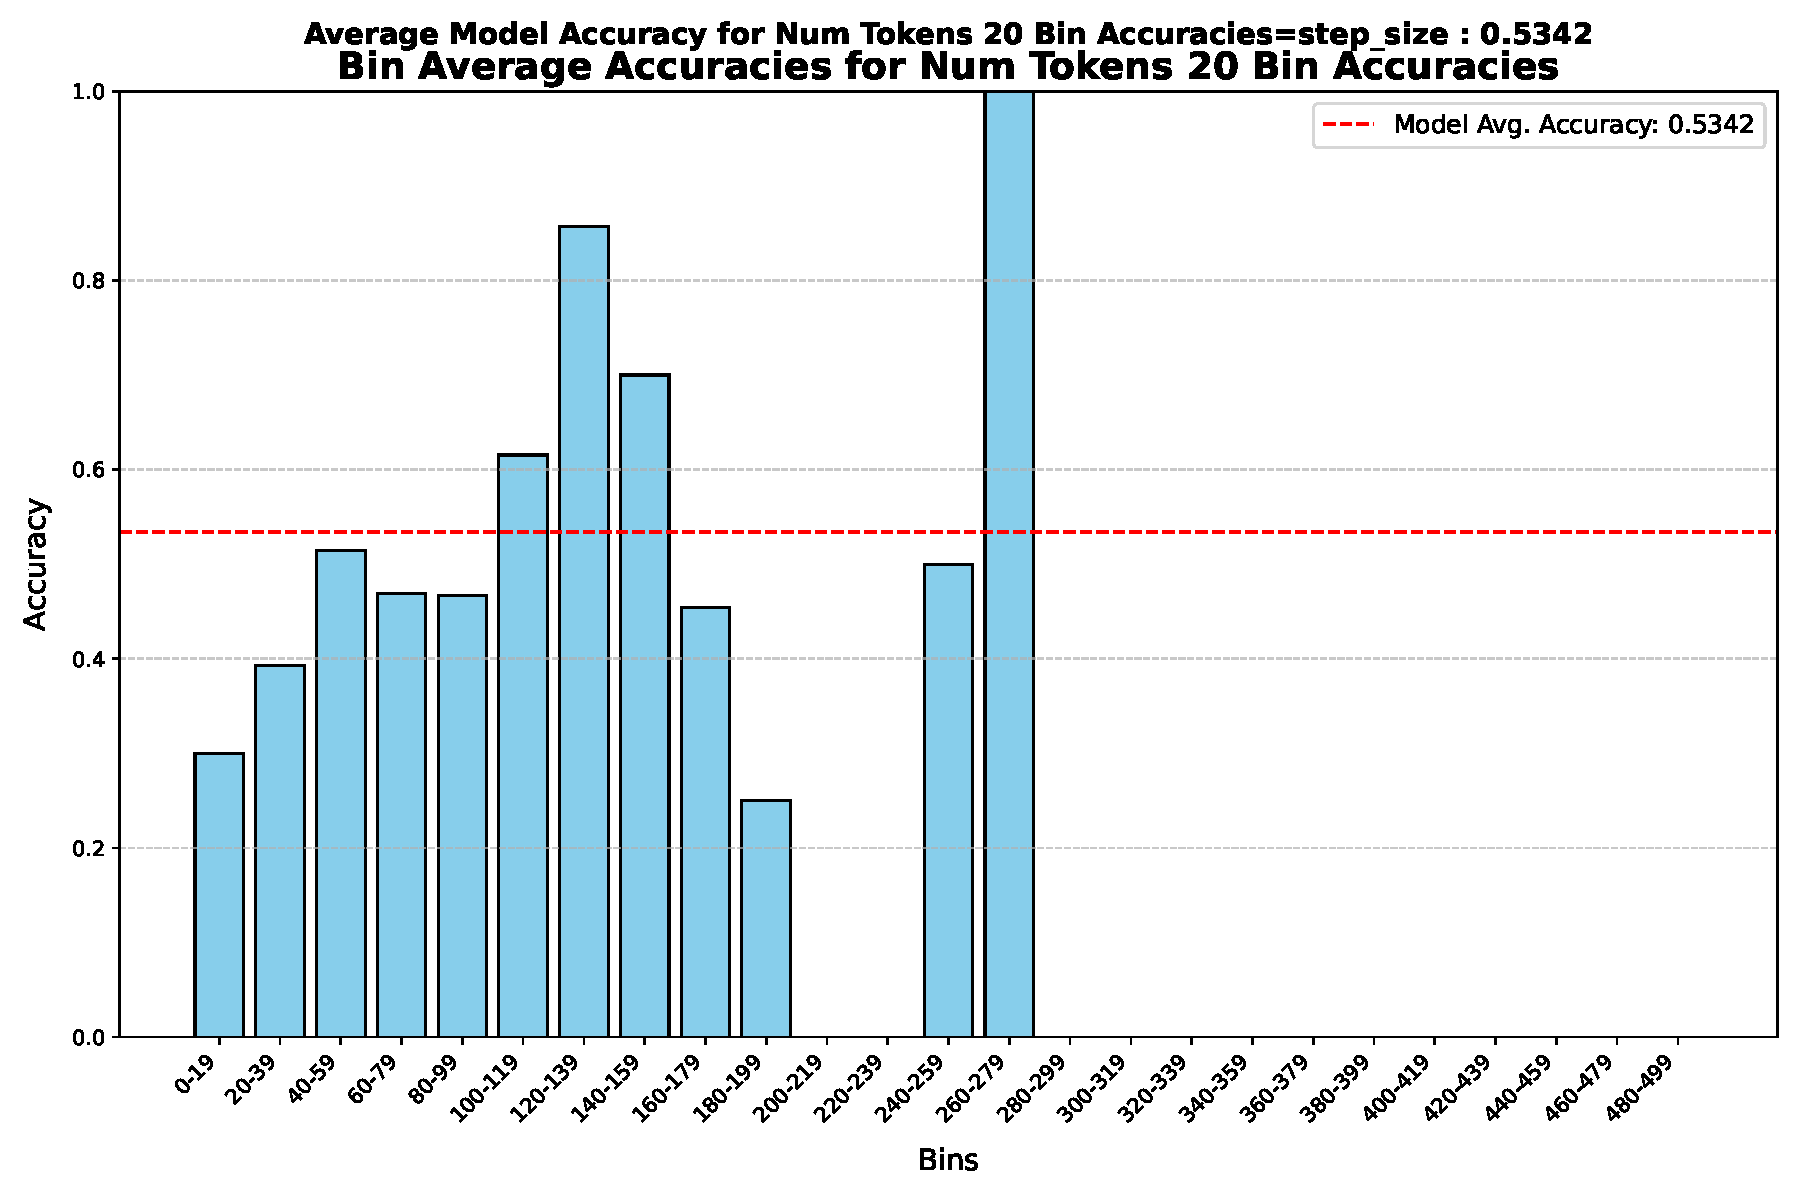
\includegraphics[width=\linewidth]{figures/attention_nn/ann_acc_num_nodes.pdf}
        \caption{Accuracy vs. number of AST nodes}
        \label{fig:ann_acc_nodes}
    \end{subfigure}
    \hfill
    \begin{subfigure}{\columnwidth}
        \centering
        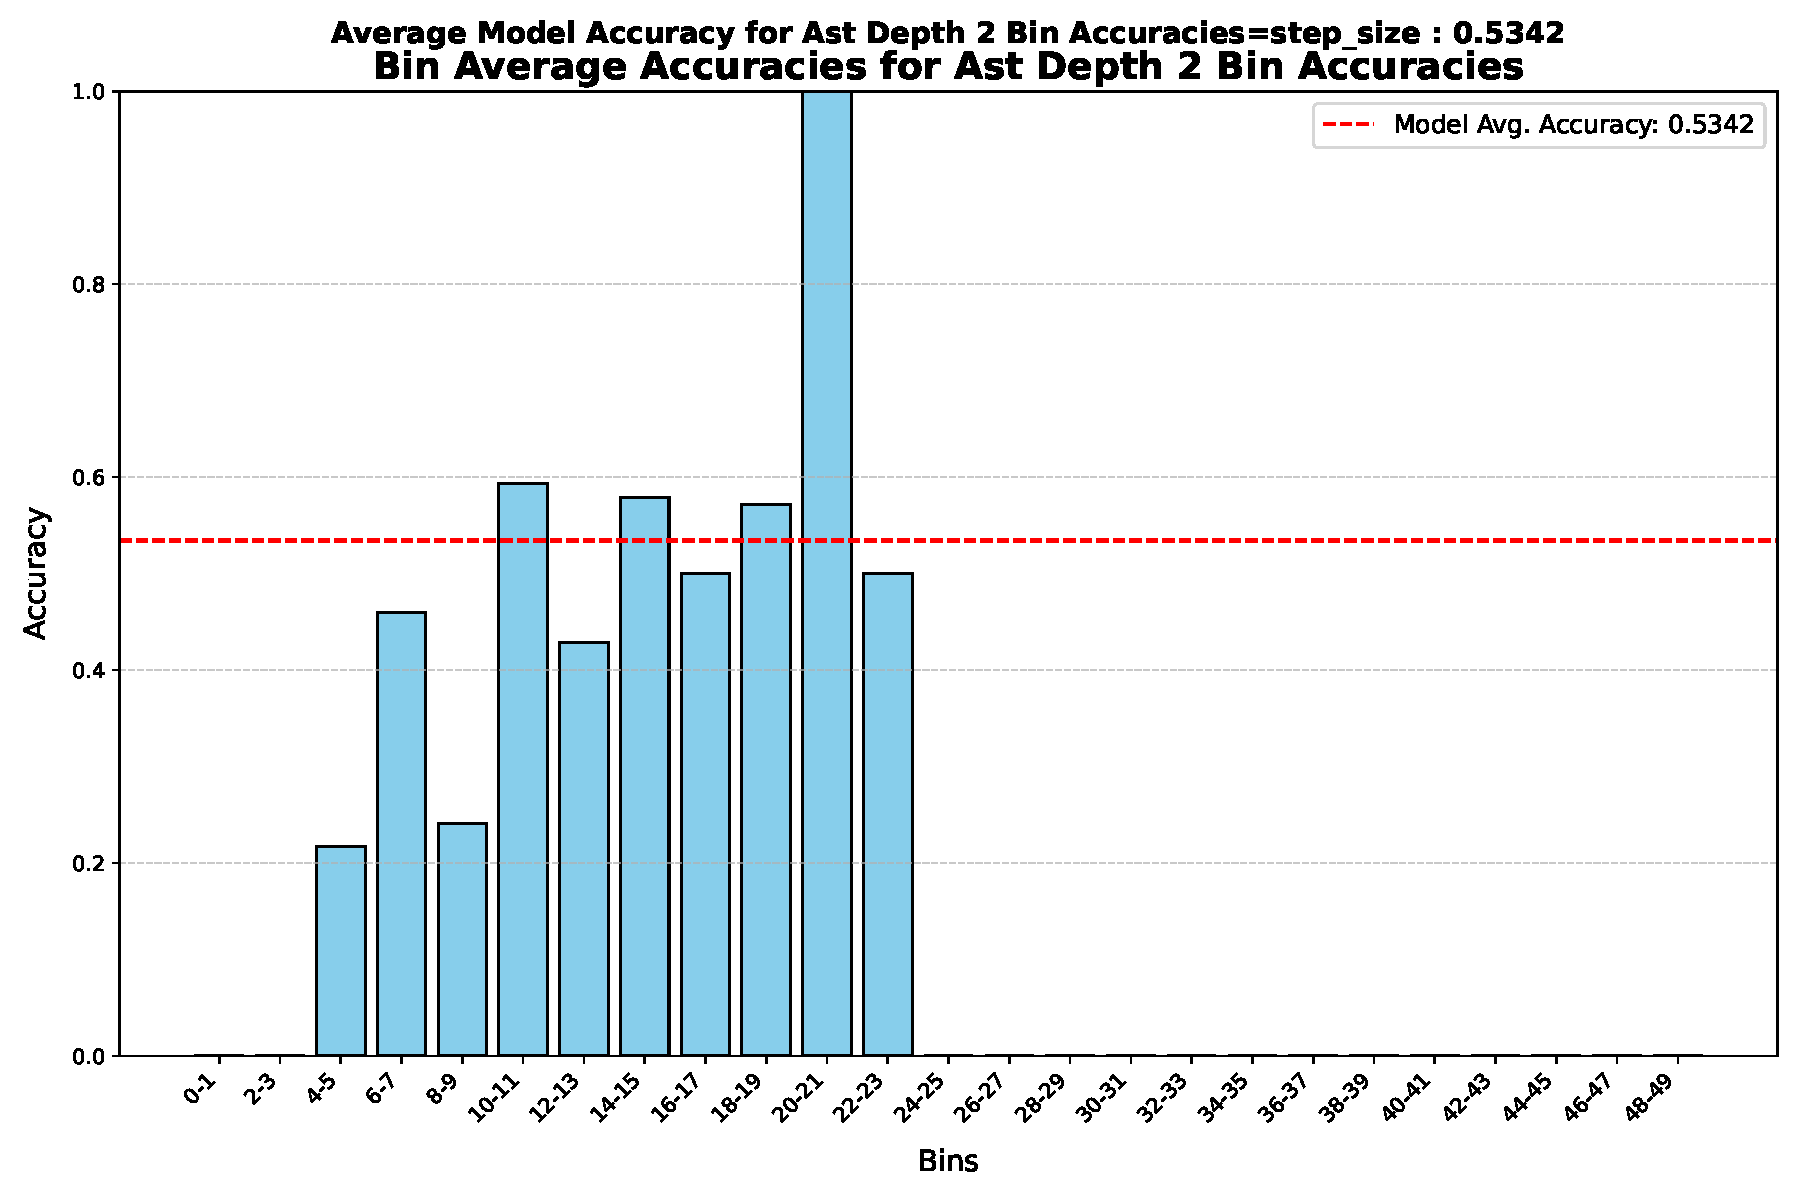
\includegraphics[width=\linewidth]{figures/attention_nn/ann_acc_depth.pdf}
        \caption{Accuracy vs. AST depth}
        \label{fig:ann_acc_depth}
    \end{subfigure}
    \caption{AttentionNN accuracy for functions with different structural complexities.}
    \label{fig:ann_acc}
\end{figure}


\section{Conclusion}

In this study, we compared traditional machine learning models and deep learning models for authorship attribution of individual functions. 
Our results showed that while BERT-based models provided the highest accuracy, they required significantly longer training times and 
computational resources. In contrast, Random Forests trained on TF-IDF representations performed surprisingly well given their simplicity 
and efficiency.

The choice of model largely depends on the trade-off between accuracy and efficiency. If the goal is purely high accuracy and computational 
resources aren’t a constraint, then BERT trained on tokenized source code is the best option. However, if speed and efficiency are more 
important, Random Forests provide a strong alternative with competitive accuracy.

We also found that different function representations significantly affect model performance. BERT struggled with AST-based pre-order 
traversal when the number of authors was high. 

AttentionNN performed better on more structurally complex functions rather than shorter ones. This highlights the need for 
careful feature selection capturing the complex relationships when applying deep learning to authorship attribution.

Overall, this study demonstrates that while deep learning methods achieve state-of-the-art performance, traditional 
machine learning approaches still hold value, especially in resource-constrained environments.



\begin{thebibliography}{00}
    \bibitem{b1} G. Eason, B. Noble, and I. N. Sneddon, ``On certain integrals of Lipschitz-Hankel type involving products of Bessel functions,'' Phil. Trans. Roy. Soc. London, vol. A247, pp. 529--551, April 1955.
    \bibitem{b2} J. Clerk Maxwell, A Treatise on Electricity and Magnetism, 3rd ed., vol. 2. Oxford: Clarendon, 1892, pp.68--73.
    \bibitem{b3} I. S. Jacobs and C. P. Bean, ``Fine particles, thin films and exchange anisotropy,'' in Magnetism, vol. III, G. T. Rado and H. Suhl, Eds. New York: Academic, 1963, pp. 271--350.
    \bibitem{b4} K. Elissa, ``Title of paper if known,'' unpublished.
    \bibitem{b5} R. Nicole, ``Title of paper with only first word capitalized,'' J. Name Stand. Abbrev., in press.
    \bibitem{b6} Y. Yorozu, M. Hirano, K. Oka, and Y. Tagawa, ``Electron spectroscopy studies on magneto-optical media and plastic substrate interface,'' IEEE Transl. J. Magn. Japan, vol. 2, pp. 740--741, August 1987 [Digests 9th Annual Conf. Magnetics Japan, p. 301, 1982].
    \bibitem{b7} M. Young, The Technical Writer's Handbook. Mill Valley, CA: University Science, 1989.
    \bibitem{b8} D. P. Kingma and M. Welling, ``Auto-encoding variational Bayes,'' 2013, arXiv:1312.6114. [Online]. Available: https://arxiv.org/abs/1312.6114
    \bibitem{b9} S. Liu, ``Wi-Fi Energy Detection Testbed (12MTC),'' 2023, gitHub repository. [Online]. Available: https://github.com/liustone99/Wi-Fi-Energy-Detection-Testbed-12MTC
    \bibitem{b10} ``Treatment episode data set: discharges (TEDS-D): concatenated, 2006 to 2009.'' U.S. Department of Health and Human Services, Substance Abuse and Mental Health Services Administration, Office of Applied Studies, August, 2013, DOI:10.3886/ICPSR30122.v2
    \bibitem{b11} K. Eves and J. Valasek, ``Adaptive control for singularly perturbed systems examples,'' Code Ocean, Aug. 2023. [Online]. Available: https://codeocean.com/capsule/4989235/tree
    \end{thebibliography}




\end{document}
